\chapter{Non-linear modelling}
\label{chp:5}

\section{Introduction}
This chapter consists of  non-linear (beyond elasticity) modelling for the Finite Element Analysis with Abaqus including VUMAT. Additionally other analytical models are proposed to make a prediction for the non-linear behaviour of FFF products. 

\section{Methods and procedures}
\subsection{Finite Element Method}
The Finite Element Analysis was conducted in Abaqus in combination with a pre-written VUMAT according to the papers proposed by Melro \cite{Melro2012InfluenceMaterials}\cite{Melro2013}\cite{Melro2013MicromechanicalModelling}. 
%explicit and implicit
Explicit simulation including plasticity with yield and failure was implemented in a similar way to Melro's code. The main difference between explicit and implicit analysis is the dependency on time and increments. For static cases without plasticity implicit is often used, for dynamic cases including plasticity explicit method is used to determine the state of the material at every increment. Implicit simulations adopt a method called Euler integration scheme which ensures stability (unconditionally stable) and facilitates larger time steps. This method may be time consuming for dynamic loads.  Explicit analyses aims to solve for acceleration. Using simplifications, the acceleration of a body can be found for every increment, and additionally the velocity and displacement. This method is not unconditionally stable, and thus smaller time increments are required. This must be smaller than the Courant time step, which dictates the time taken by a sound wave to travel across an element. Explicit analysis offers a faster solution in events where there is a dynamic equilibrium. Since implicit has more trouble with non-linear material behaviour (as is plasticity) an explicit method was used \cite{ImplicitMethod}.
%Explanation of the VUMAT code

A VUMAT subroutine code was used in combination with ABAQUS to adjust constitutive models. A VUMAT is used if the abaqus material model library does not represent the behaviour of the material well, or if a user wants a more accurate response in a complex situation\cite{SimuliaWriting}. Considering the very limited commercial models available for polymers, an adjusted VUMAT was implemented to simulate this behaviour. The VUMAT is written in academic coding language FORTRAN and makes use of inputs for material properties, and outputs Solution Dependant Variables, which can be displayed by the Abaqus interface. The VUMAT requires hardening curves as a input to determine the plasticity behaviour of the material, these hardening curves need to be extracted from uniaxial tension and compression data. For this study the tensile experimental data is extracted from the filament tensile tests as is presented in chapter 5. The compressive curve is of less importance, since our simulations will be focused on uni-axial tensile loading cases. However, the yield function as is presented in equation \ref{eqn:yieldpolymers} is strongly dependant on the yield stress in compression, therefore an approximation for the hardening curve in compression is needed. Wang et al. \cite{Wang2016ExperimentalRates} proposed an extensive study on the compressive behaviour of PC/ABS, one of the curves from this work is used as the compressive input curve. 

Before implementing the hardening curve, the curve needs to be converted from normal strain to plastic strain, with the following equation:
\begin{equation} \label{eqn:toplastic}
\epsilon_{1p}=\epsilon_{1t}-\epsilon_{1e}
\end{equation}
Where $\epsilon_{1p}$ is the plastic strain, $\epsilon_{1t}$ is the total strain and $\epsilon_{1e}$ is the elastic strain, which follows the regular $\sigma/E$ relation. The corresponding hardening curves are shown in figure \ref{fig:hardening}, and are subtracted from the filament stress strain curves presented in chapter 5.

\begin{figure}[H]
    \centering
    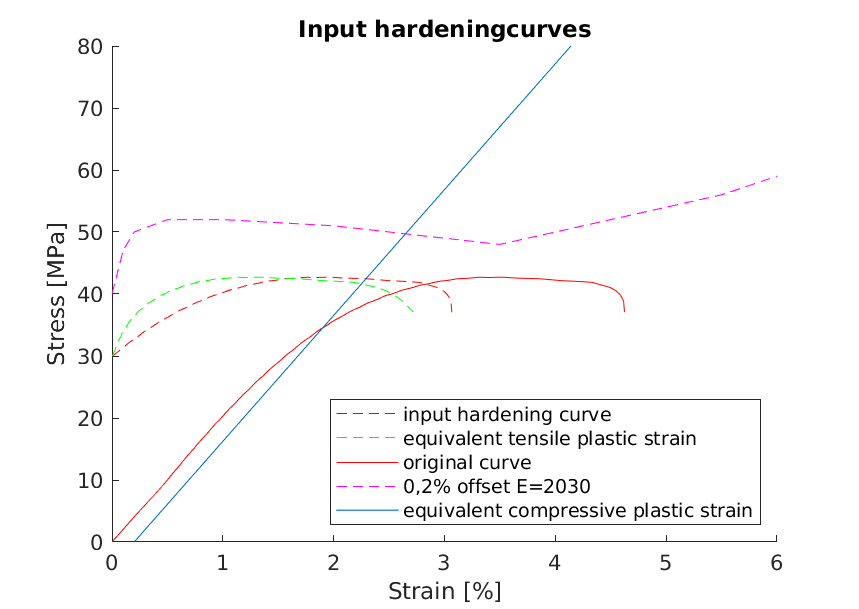
\includegraphics[width=0.60\textwidth]{chapter_7_non-elasticmodelling/figures/Hardening.png}
    \caption{Implemented hardening curves for Ultimaker ABS}
    \label{fig:hardening}
\end{figure}

The 0.2\% offset is used to indicate the yield point that would be defined for metals. The "anelastic" point (the point where linear elasticity practically ends and  where the hardening curve starts) is near this 0.2\% offset point. 

%explenation MATLAB code

Similar to the elastic modelling code, MATLAB is used to provide the input parameters and geometric shape. For the explicit method no periodic boundary conditions are applied, this would require too much computational power to run. In return, a convergence study is carried out for multiple stacked RVEs besides a convergence study for mesh sensitivity. 
%Load conditions. 
The mesh is loaded in the different loadcases, uniaxial tension in 1, 2 and 3 direction. The RVE is constrained on one face and loaded with a velocity boundary of equal to the $(a/20)/s$ where $a$ is the length of the perpendicular edge with respect to the loading face. This results in a effective strain percentage of 5\% after 1 second. 
%Running the code
When the appropriate ABAQUS input files are generated by the MATLAB code, and the VUMAT file is defined alongside with the corresponding harderning curves, the job is submitted trough the unix shell to the kernel.
%Method of the code
For testing the constitutive model defined in the VUMAT a one element test was performed to asses the material response. The subroutines in VUMAT deterimes after every increment what the stress state is in the element, and what behaviour the element is coded to display. For the first region of the load, the element will behave elastically, up to the increment where the yield function defined by Tjoegbl (equation \ref{eqn:yieldpolymers}) is surpassed. At this moment the element behaves plastically and will follow the implemented hardening curve through an integration algorithm, which is described in more detail in Melro's paper \cite{Melro2013MicromechanicalModelling}.  Additionally the subroutine checks if the strain based Johnson Cook failure model is surpassed according to the defined Johnson Cook variation presented in equation \ref{eqn:JC}. This criterion implements an uniaxial tension strain to determine an equivalent strain that needs to be met before the element starts to fail. After this moment the element is deleted and will not exhibit any stiffness. 
In a larger model consisting of multiple elements, the geometry will create stress concentration points where elements will premature yield and fail. This will cause a crack to grow and finally will lead to fracture. The goal of the simulation is to determine the effect the geometry has on the macroscopic response of the RVE, that is, the reactional force opposite from the load face.
In a model consisting of multiple elements this subroutine is repeated for every element trough every increment. This RVE has more than 30000 elements and can go up to more than 300000 increments, resulting in running the subroutine more than $9*10^{10}$ times. This requires extensive computational power, therefore the High Performing Computing cluster of the TU Delft is used to perform this explicit analysis. Using the capabilities of one of the nodes in this computer, the simulation for each loading case took more than 4 hours in general.

The goal of the FEM simulation is to predict the stress strain response in the 3 principle directions and to compare these with the empirical tests. Additionally, different aspect ratios of the RVE as is discussed in chapter 4 can be simulated. But first a convergence study should be conducted to determine the accuracy of the simulations.
%mesh convergeance

When the FEM simulation finished, an ODB file is generated including the requested field and history output of certain time intervals. This includes i.a. the different types of stresses and strains etc. in the nodes and elements. The reaction forces (the amount of force a node "feels" when subjected to a load when it has no degrees of freedom) are prompted for the nodes. The nodes at the constrained face will generate enough information to determine the stress strain response of a certain load according to the following equation: 

\begin{equation} \label{eqn:RVESS}
1/A_{face}*\sum_{n=1} n_{face}
\end{equation}where $A_{face}$ is the surface of the constrained face and $n_{face}$ are the nodes at the constrained face. 

\subsection{Convergence study}
To determine the mesh sensitivity a convergence study is conducted. The same meshing strategy, including the partitioning, was implemented as is presented in chapter 6. Element sizes of 0.004 0.006 0.008 and 0.01 mm are tested for the 3 directions for an aspect ratio of 0.5. The different forms of meshes are presented in figure \ref{fig:meshes}

\begin{figure}
\centering
  \begin{subfigure}[b]{0.48\textwidth}
    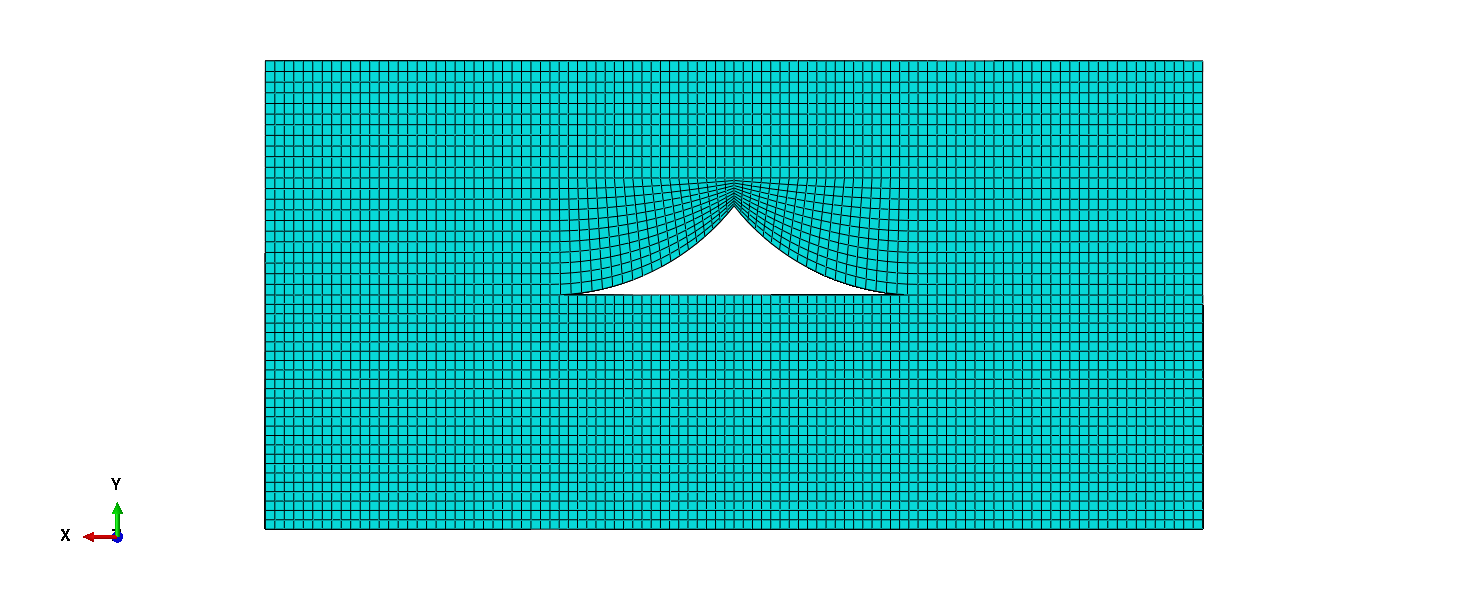
\includegraphics[width=\textwidth]{chapter_7_non-elasticmodelling/figures/mesh0004.png}
    \caption{ mesh 0.004}
  \end{subfigure}
  %
  \begin{subfigure}[b]{0.48\textwidth}
    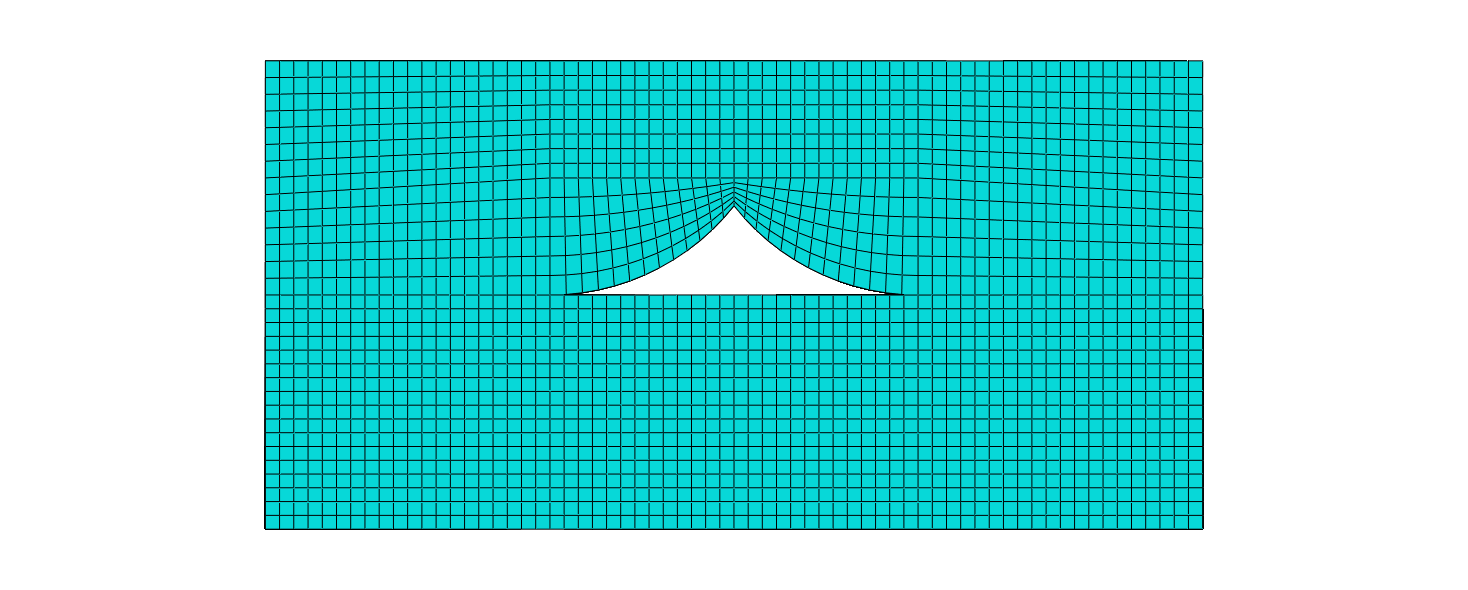
\includegraphics[width=\textwidth]{chapter_7_non-elasticmodelling/figures/mesh0006.png}
    \caption{ mesh 0.006}
  \end{subfigure}
  \\
    \begin{subfigure}[b]{0.48\textwidth}
    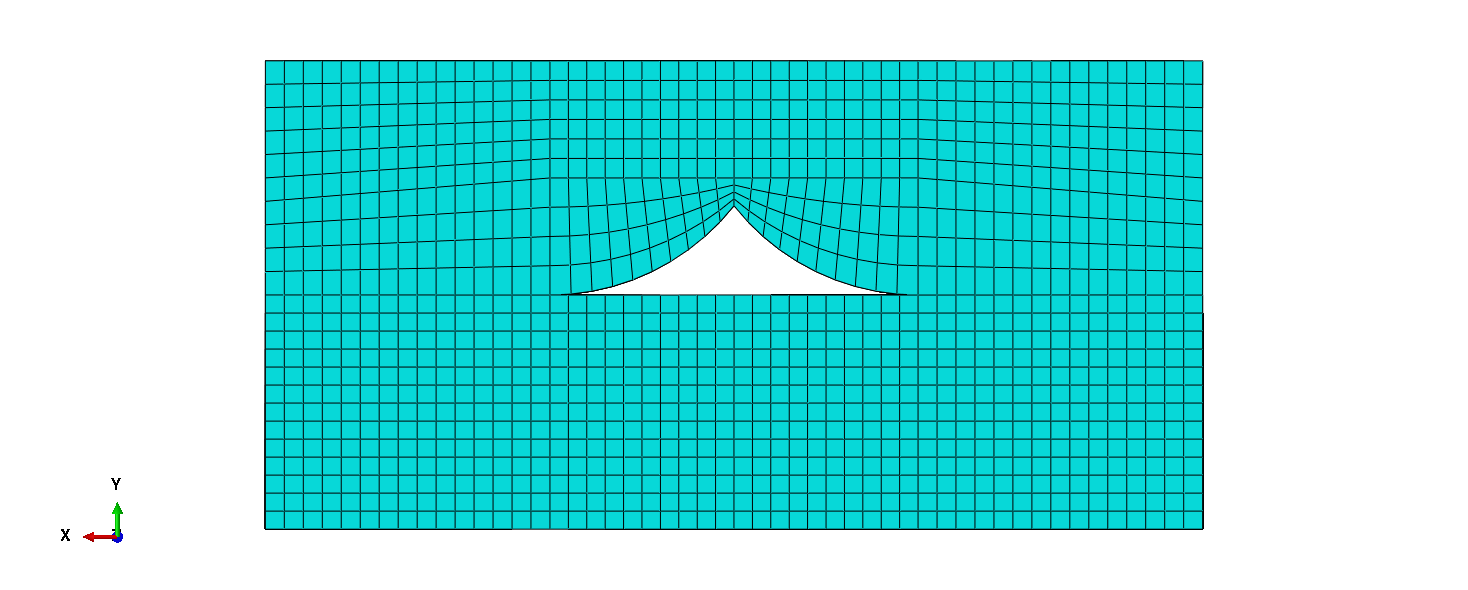
\includegraphics[width=\textwidth]{chapter_7_non-elasticmodelling/figures/mesh0008.png}
    \caption{ mesh 0.008}
  \end{subfigure}
  %
  \begin{subfigure}[b]{0.48\textwidth}
    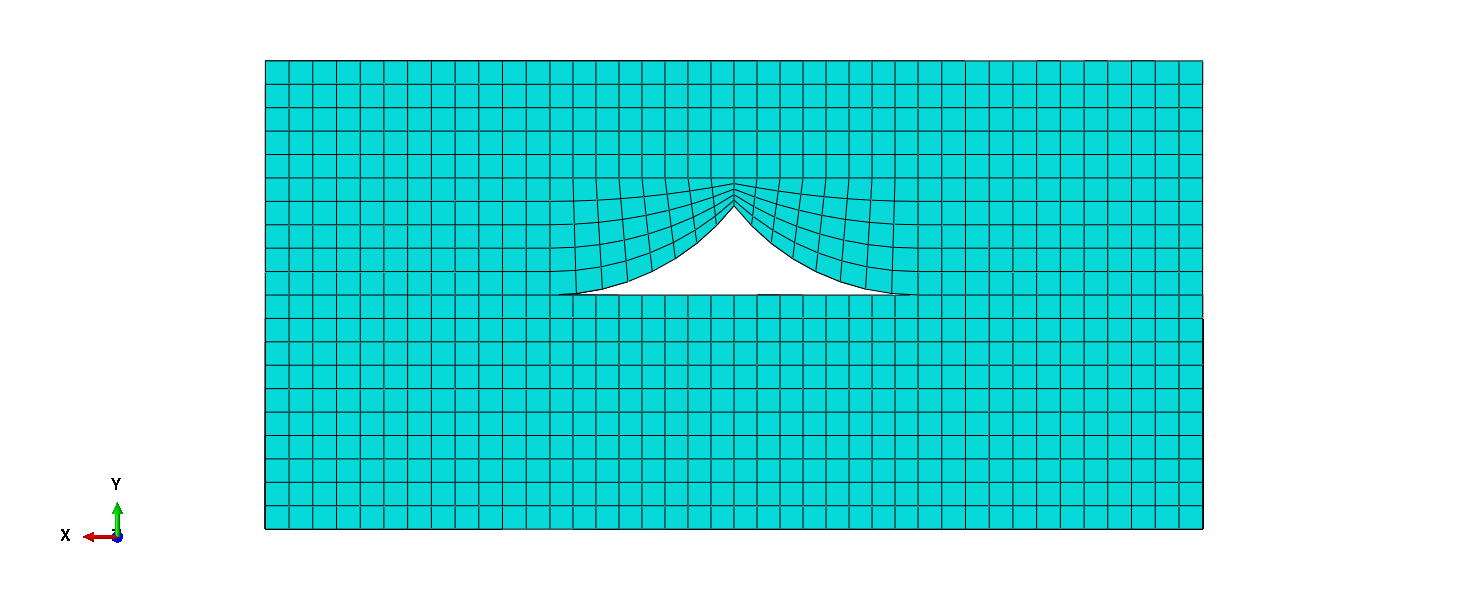
\includegraphics[width=\textwidth]{chapter_7_non-elasticmodelling/figures/mesh001.png}
    \caption{ mesh 0.01}
  \end{subfigure}
  \\
  
  \caption{Different element sizes implemented for convergence study.}
  \label{fig:meshes}
\end{figure}

Additionally, a convergence study is conducted for multiple connected RVEs. Four stacked RVEs in the XY and ZX planes are analyzed and additionally a block of 2 x 2 x 2 RVEs is simulated. The RVEs are produced with a aspect ratio of 0.5 and with an element size of 0.01, similar to the generation of the RVE for the elastic analysis. The RVE combinations can be seen in figure \ref{fig:mulRVE}.

\begin{figure}
\centering
  \begin{subfigure}[b]{0.48\textwidth}
    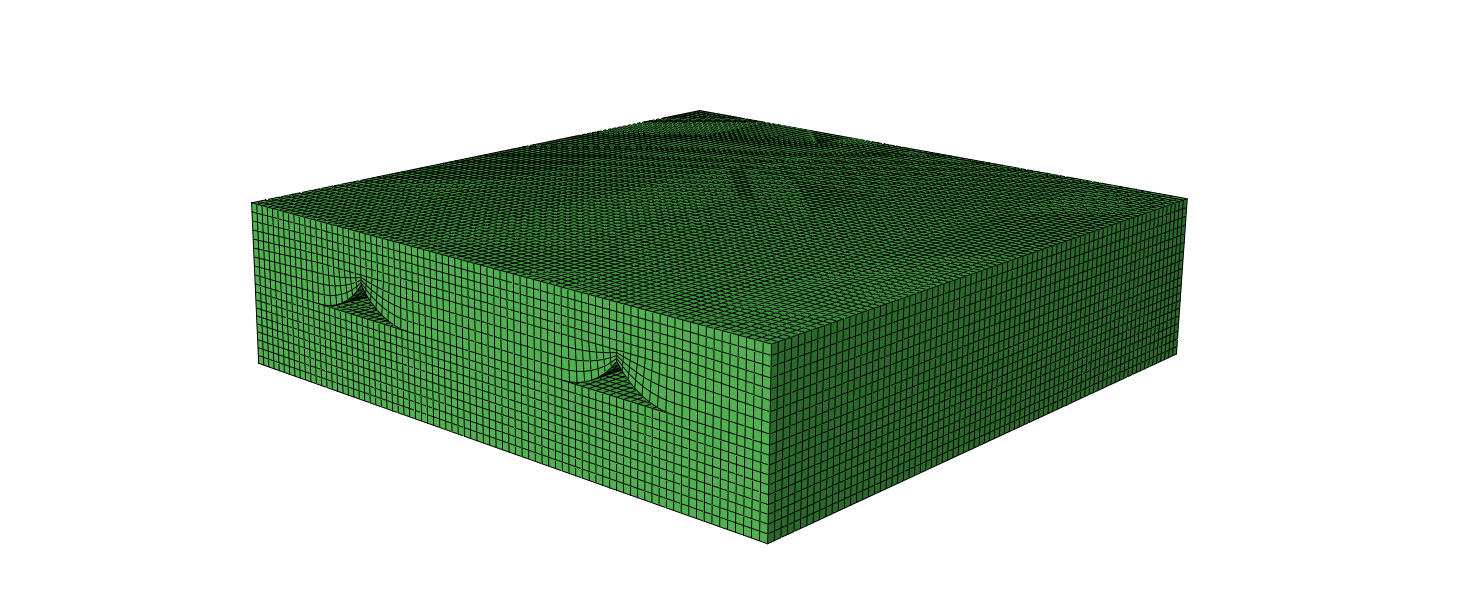
\includegraphics[width=\textwidth]{chapter_7_non-elasticmodelling/figures/RVEXY.png}
    \caption{ RVE XY plane}
  \end{subfigure}
  %
  \begin{subfigure}[b]{0.48\textwidth}
    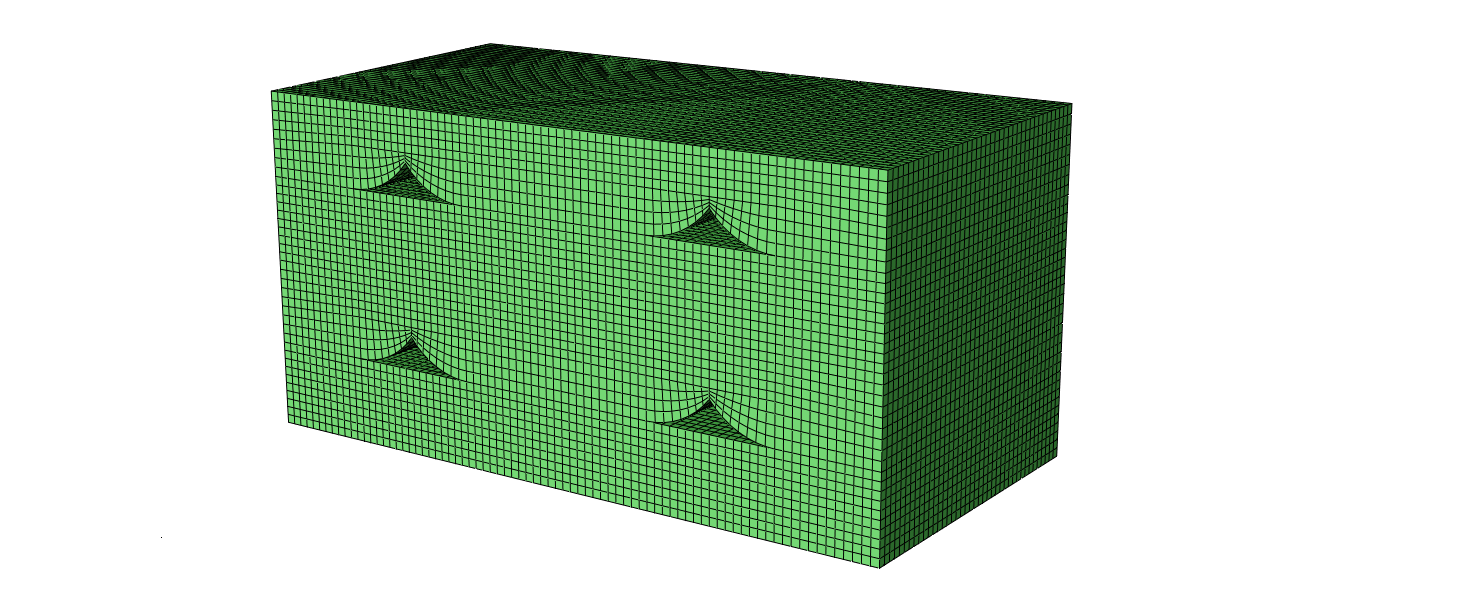
\includegraphics[width=\textwidth]{chapter_7_non-elasticmodelling/figures/RVEZX.png}
    \caption{ RVE ZX plane}
  \end{subfigure}
  \\
    \begin{subfigure}[b]{0.48\textwidth}
    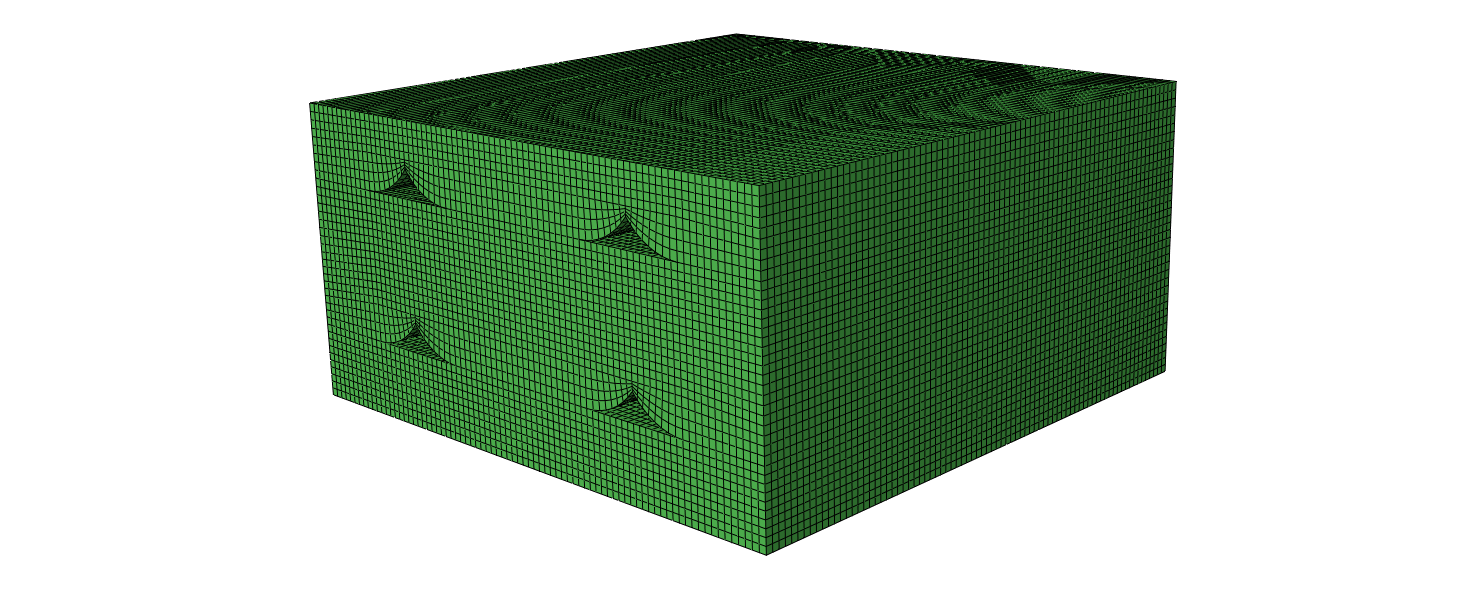
\includegraphics[width=\textwidth]{chapter_7_non-elasticmodelling/figures/RVEZYX.png}
    \caption{ RVE ZYX direction }
  \end{subfigure}
  %
  
  \caption{Different RVE duplicates implemented for convergence study.}
  \label{fig:mulRVE}
\end{figure}

\subsection{Stress Intensity approach}
An additional approach was investigated with respect to the failure mechanism in the RVE. As is described in chapter 2, linear elastic fracture mechanics states that the critical failure stress can be predicted if the form and size of a crack is known. The equation for the stress intensity factor can be seen in equation \ref{eqn:criticalstress}. The periodic voids can be assumed as cracks for a plane strain loading condition in the 2 and 3 direction, which are dependant on the line thickness and width. With these parameters a critical stress $(\sigma_c)$ can be found which should give an approximation for the failure stress in FFF produced parts. 

Additionally, the cracktip plasticity theory, explained in chapter 2 is used to predict the radius of the plastic deformation. This is useful to predict the plastic behaviour involved in the failure of parts. Products that show low plasticity in their fracture surface are suspected to have a low toughness at the fracture surface, resulting in brittle failure, which might be caused by improper failure. To have a better understanding of the size of the cracktip plasitcity, the radius of plasticity is plotted against the distance between the crack tip and the edge of the RVE. These lengths are not equal in the 3 direction, therefore the average of both lengths is used to determine the distance between two cavities. 

\section{Results}
\subsection{Convergence study mesh}
The convergence study of the mesh for mesh sizes 0.004, 0.006, 0.008 and 0.01 with an RVE with aspect ration 0.5 is presented in figure \ref{fig:meshconv}. The 3 principal directions are presented consecutively in green, red and blue. For some mesh sizes the simulations were unsuccessfully (0.004 in 1 and 2 direction and 0.006 in 1 direction), the simulations in the 3 direction give a representative view on the mesh sensitivity.  

\begin{figure}[H]
    \centering
    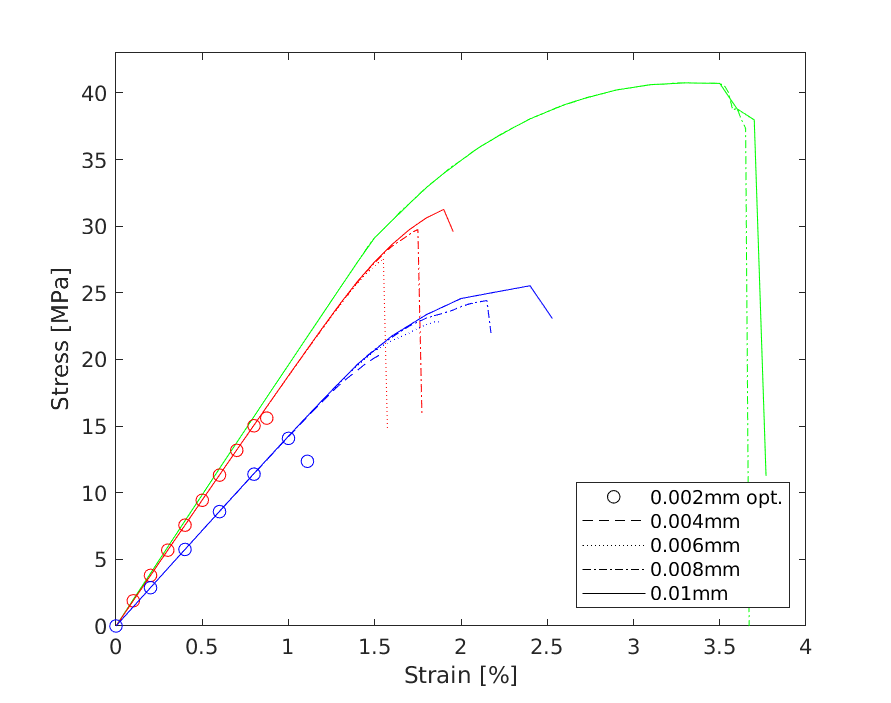
\includegraphics[width=0.60\textwidth]{chapter_7_non-elasticmodelling/figures/meshconv.png}
    \caption{Convergence study for different mesh sizes}
    \label{fig:meshconv}
\end{figure}

\subsection{Convergence study RVEs}
The convergence study for the RVE duplicates are presented in figure \ref{fig:RVEgraph}, and are related to the figures is figure \ref{fig:mulRVE}. Here the ZYX RVE in the 1 principal direction failed, the other results give a good representation of the sensitivity of the multiple RVEs. 

\begin{figure}[H]
    \centering
    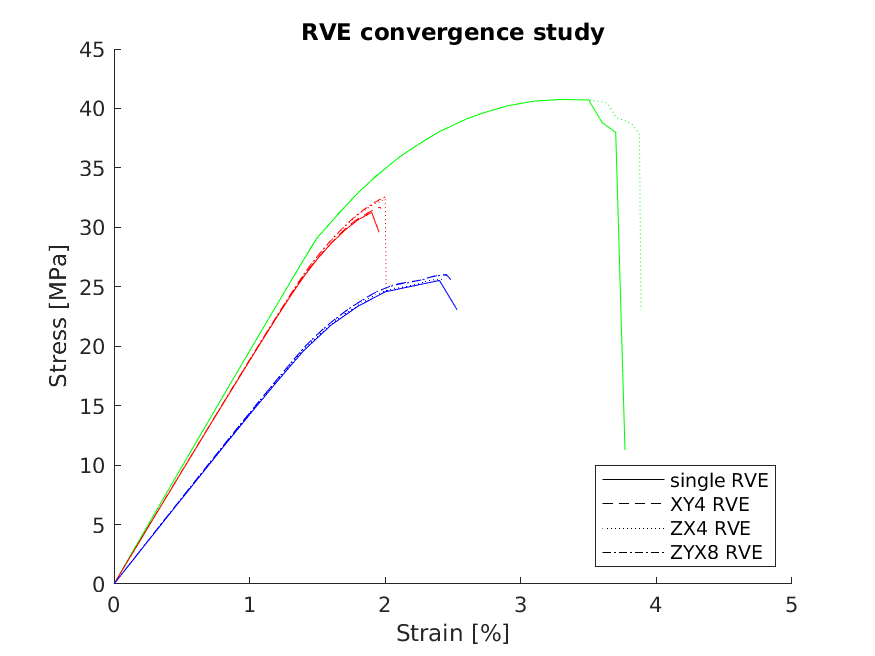
\includegraphics[width=0.60\textwidth]{chapter_7_non-elasticmodelling/figures/RVEconv.png}
    \caption{Convergence study for RVE duplicates}
    \label{fig:RVEgraph}
\end{figure}

\subsection{Simulations compared with empirical results }
In figure \ref{fig:ComparisonSS} the 0.5 aspect ratio simulation with a 0.008 element mesh is compared with the empirical results from the 0.4 x 0.2 ASTM 3039 tensile test samples presented in chapter 5. 

\begin{figure}[H]
    \centering
    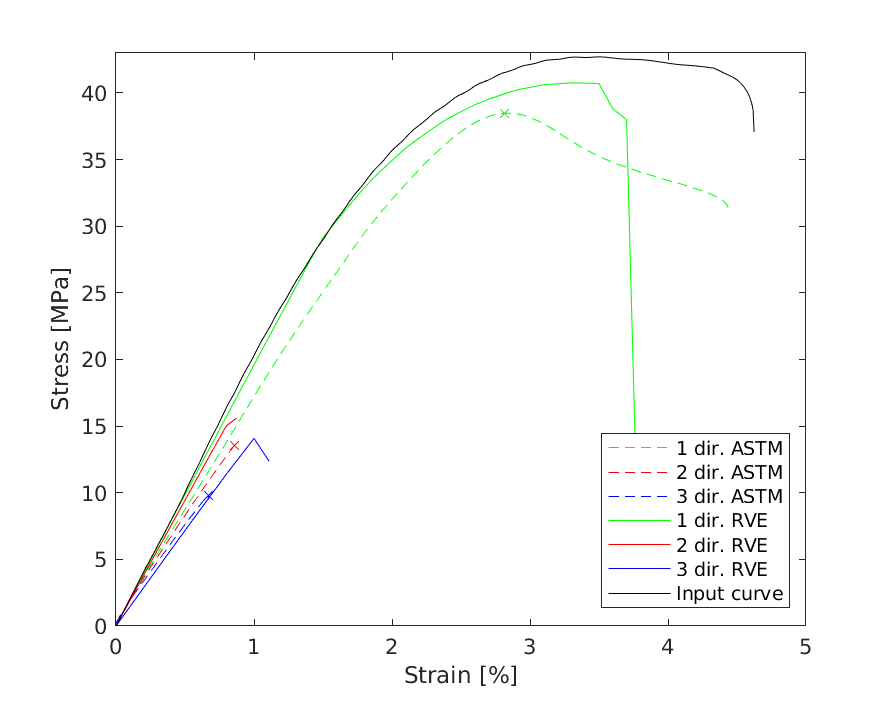
\includegraphics[width=0.60\textwidth]{chapter_7_non-elasticmodelling/figures/ComparisonSS.png}
    \caption{Comparison between the empirical obtained results and the simulated RVE in the 3 principle directions}
    \label{fig:ComparisonSS}
\end{figure}

\subsection{Simulations with altering aspect ratio}
In the following figures \ref{fig:AR1},\ref{fig:AR2},\ref{fig:AR2} the dependency on the aspect ratio is shown for a mesh with an element size of 0.01. Aspect ratios of 0.125, 0.2, 0.25, 0.5, 0.75 and 1 are simulated for the 3 principle directions. 

\begin{figure}[H]
    \centering
    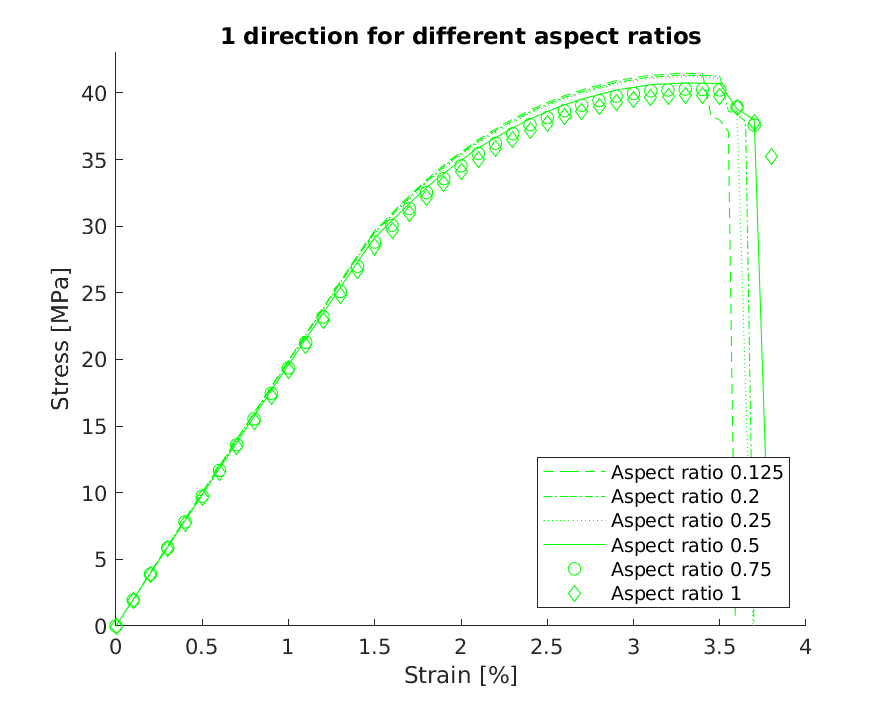
\includegraphics[width=0.60\textwidth]{chapter_7_non-elasticmodelling/figures/AR1.png}
    \caption{Comparison between different aspect ratios in the 1 direction}
    \label{fig:AR1}
\end{figure}
\begin{figure}[H]
    \centering
    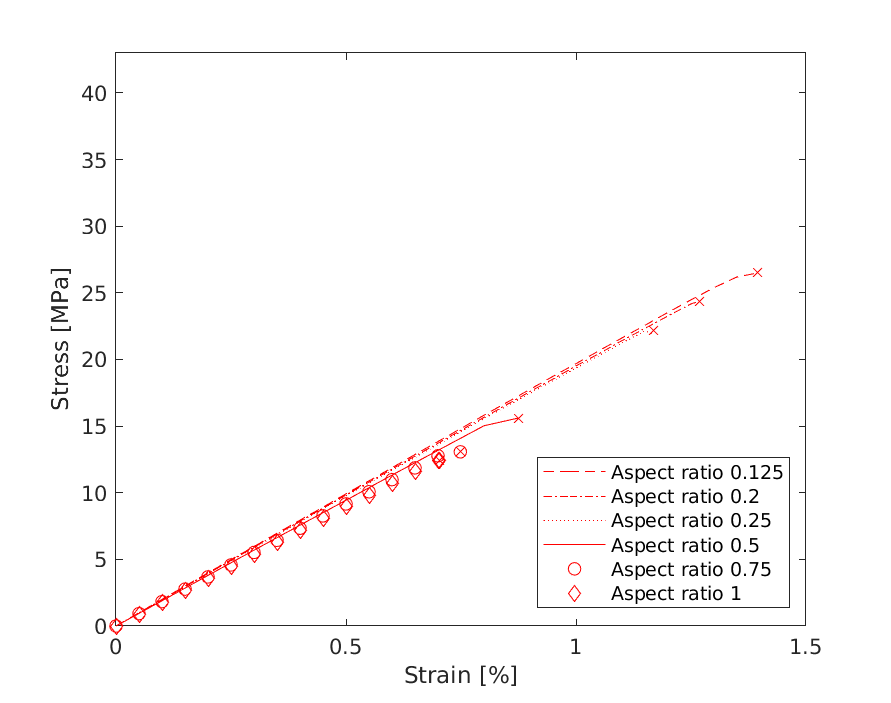
\includegraphics[width=0.60\textwidth]{chapter_7_non-elasticmodelling/figures/AR2.png}
    \caption{Comparison between different aspect ratios in the 2 direction}
    \label{fig:AR2}
\end{figure}
\begin{figure}[H]
    \centering
    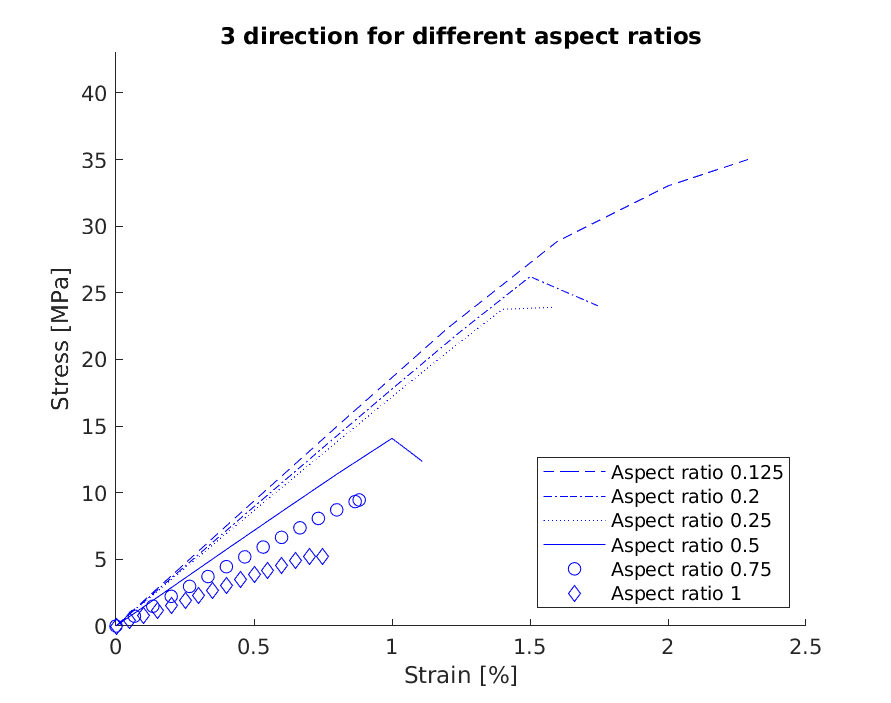
\includegraphics[width=0.60\textwidth]{chapter_7_non-elasticmodelling/figures/AR3.png}
    \caption{Comparison between different aspect ratios in the 3 direction}
    \label{fig:AR3}
\end{figure}
\subsection{Contour plots of different aspect ratios }
The following figures (\ref{fig:Contourplot} will present the contour plots at the moment before failure of the maximum equivalent total strain of the 3 principal directions for the aspect ratios of 0.125, 0.5 and 1. Since the Johnson Cook model is implemented based on a equivalent total strain of 0.0606 in tensile, this will give a decent representation of the region of failure. Note that the Johnson Cook criterion is dependant on the stress triaxiality, this means that the equivalent total strain at fracture can be higher or lower than the implemented uni-axial fracture strain of 0.0606 for complex strain states.

\begin{figure}
\centering
  \begin{subfigure}[b]{0.6\textwidth}
    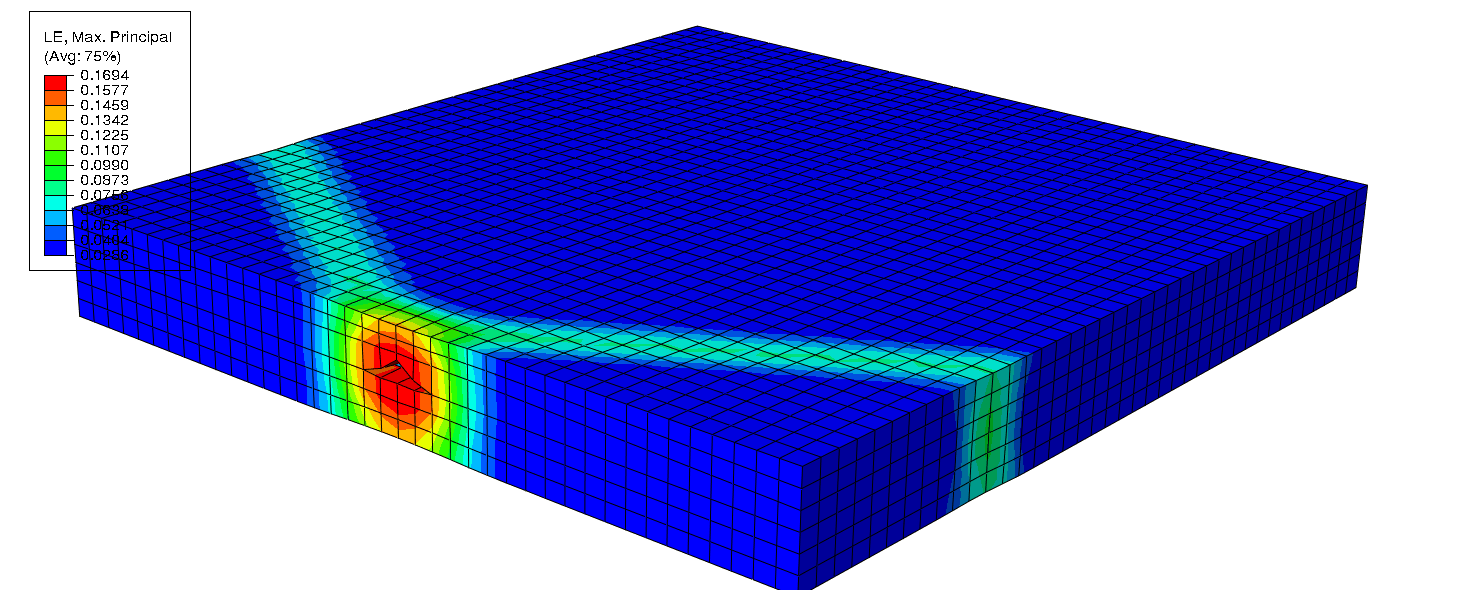
\includegraphics[width=\textwidth]{chapter_7_non-elasticmodelling/figures/0125p1.png}
    \caption{0.125 aspect ratio, 1 direction}
  \end{subfigure}
  \\
  \begin{subfigure}[b]{0.6\textwidth}
    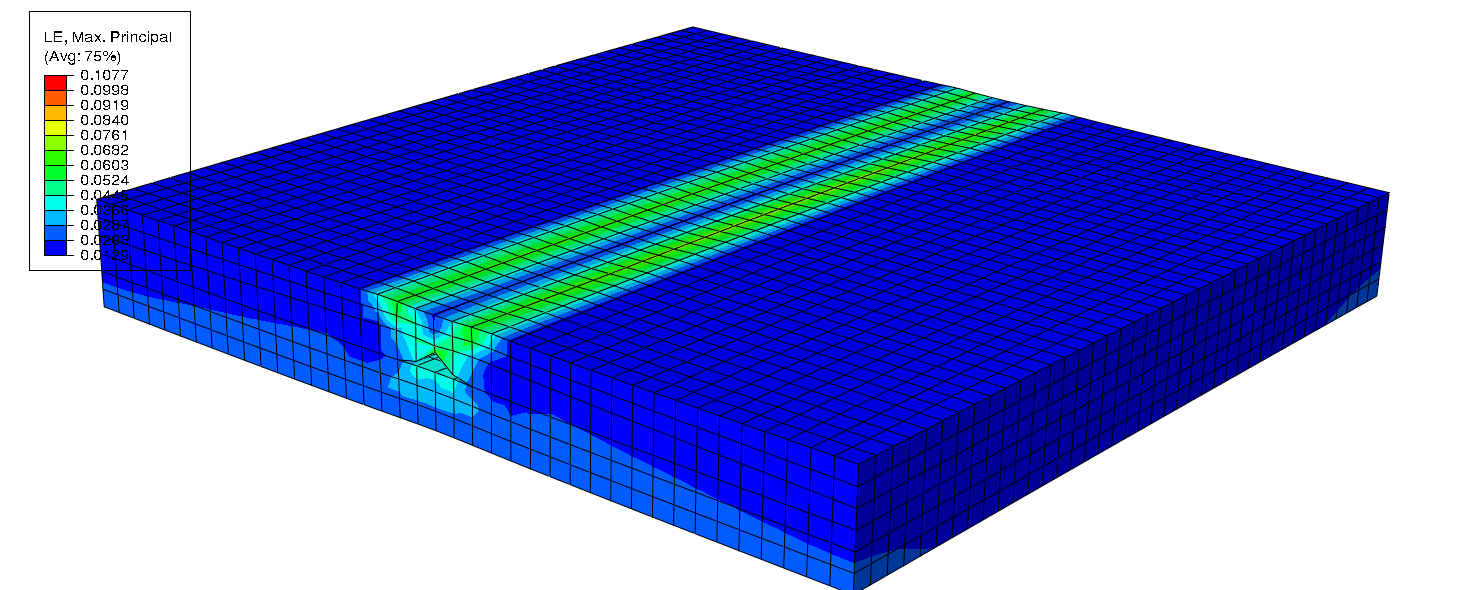
\includegraphics[width=\textwidth]{chapter_7_non-elasticmodelling/figures/0125p2.png}
    \caption{0.125 aspect ratio, 2 direction}
  \end{subfigure}
  \\
    \begin{subfigure}[b]{0.60\textwidth}
    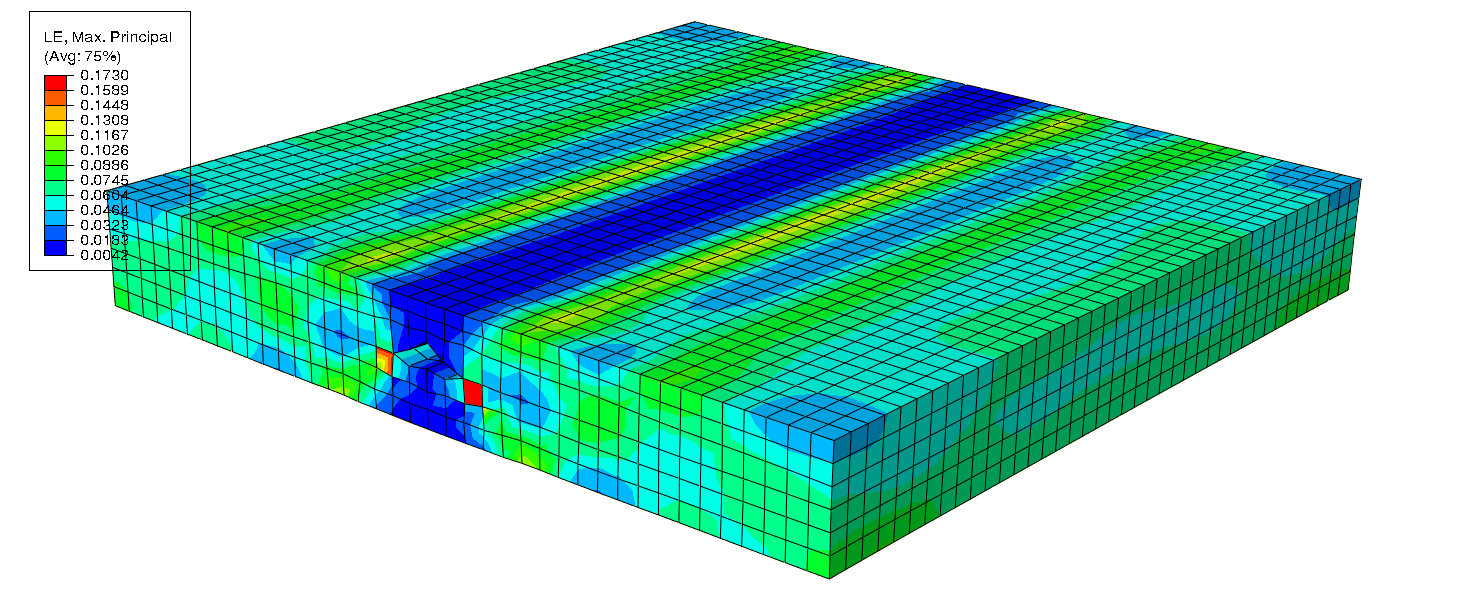
\includegraphics[width=\textwidth]{chapter_7_non-elasticmodelling/figures/0125p3.png}
    \caption{0.125 aspect ratio, 3 direction}
  \end{subfigure}
  \\
  \begin{subfigure}[b]{0.70\textwidth}
    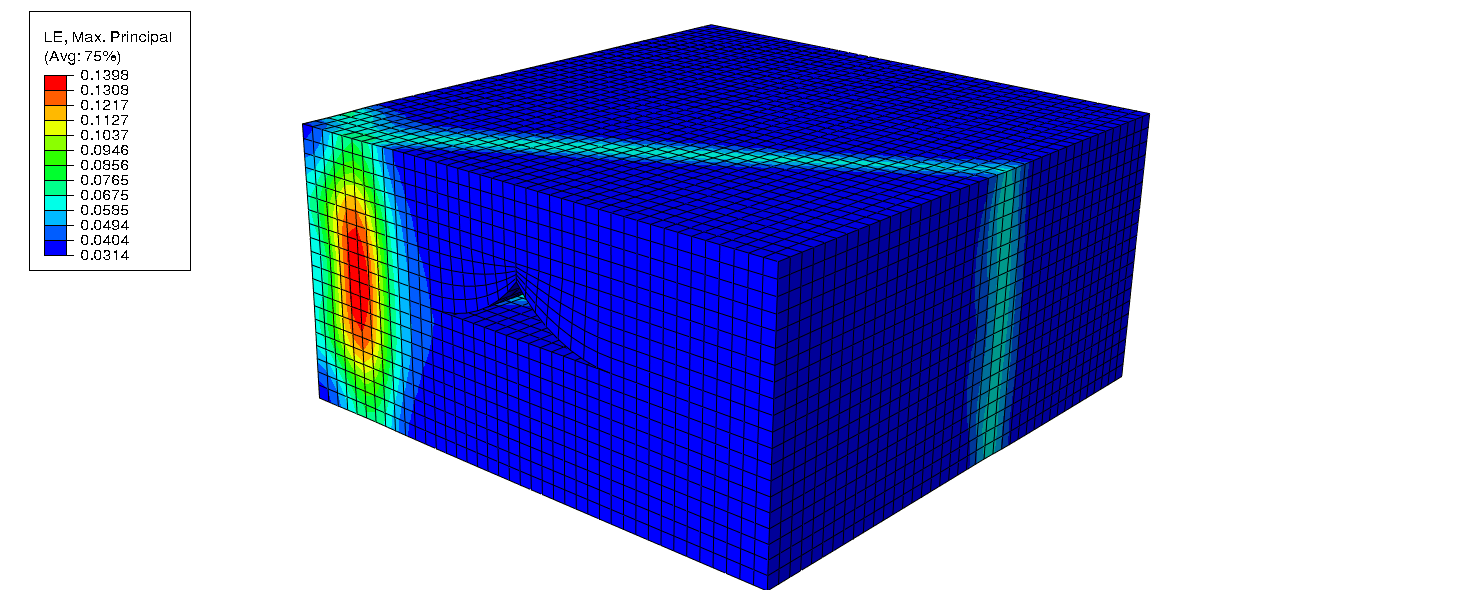
\includegraphics[width=\textwidth]{chapter_7_non-elasticmodelling/figures/05p1.png}
    \caption{0.5 aspect ratio, 1 direction}
  \end{subfigure}
  \\
    \begin{subfigure}[b]{0.70\textwidth}
    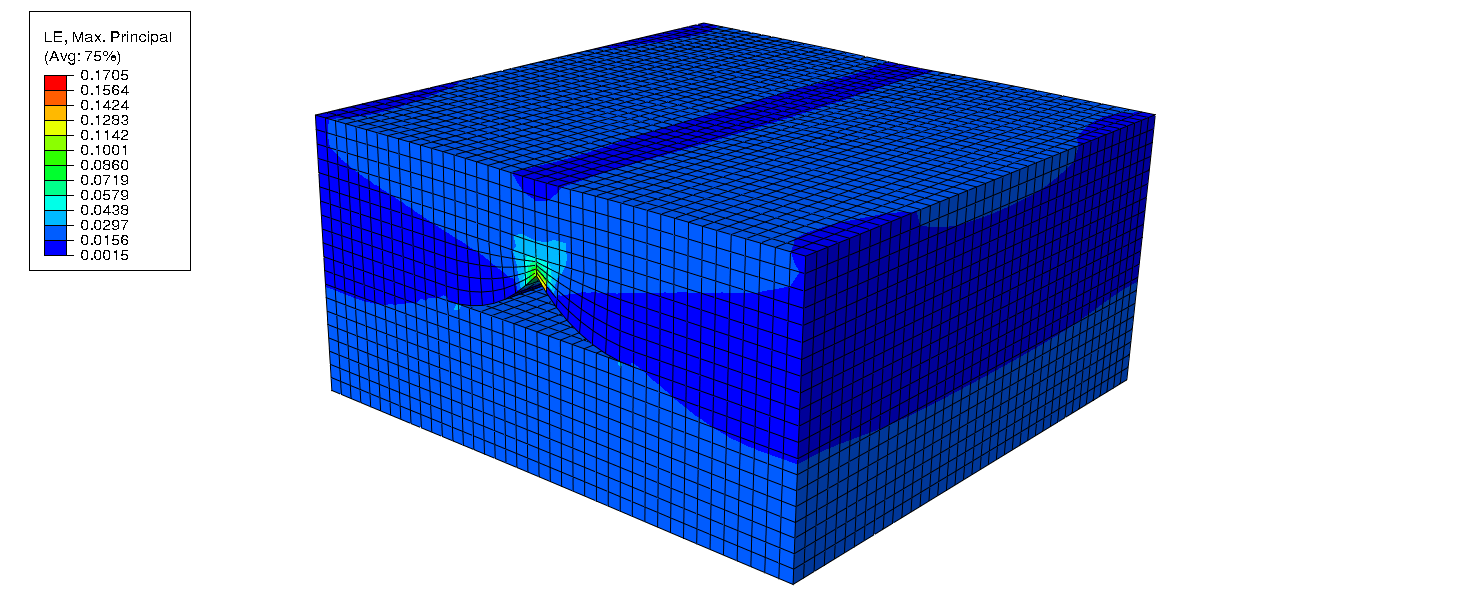
\includegraphics[width=\textwidth]{chapter_7_non-elasticmodelling/figures/05p2.png}
    \caption{0.5 aspect ratio, 2 direction}
  \end{subfigure}
  \end{figure}
  \\
    \begin{figure}
    \centering
  \begin{subfigure}[b]{0.70\textwidth}
    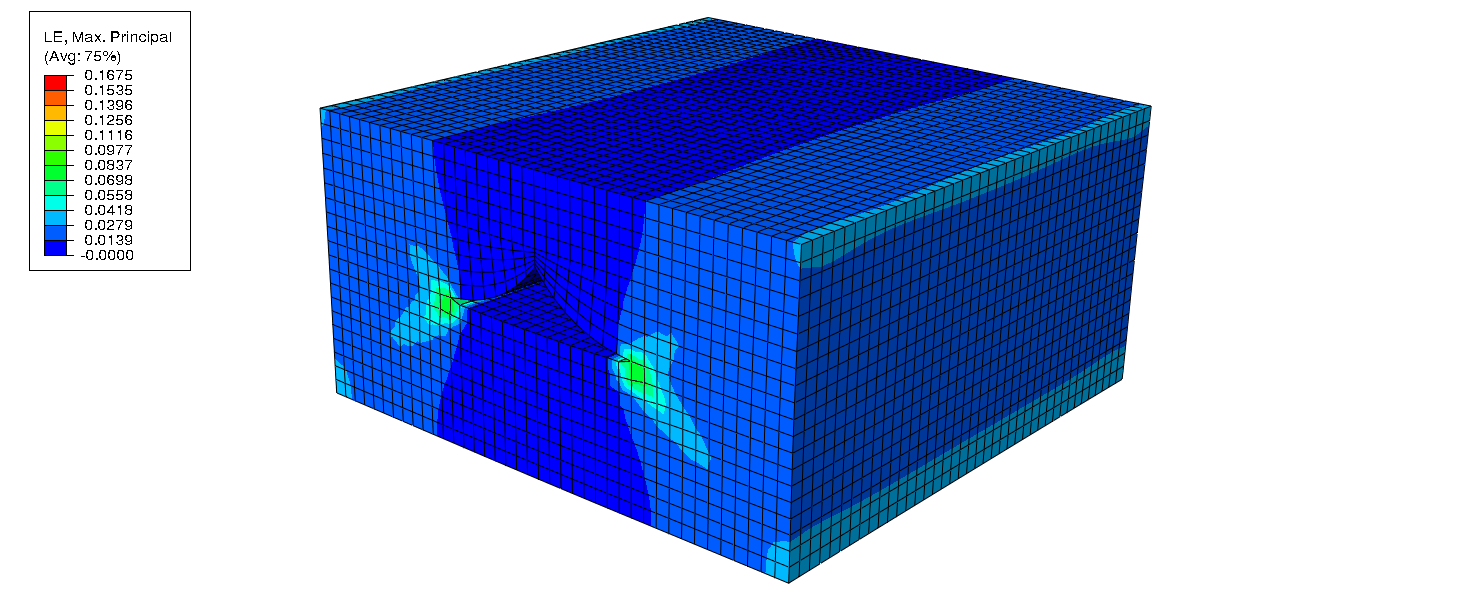
\includegraphics[width=\textwidth]{chapter_7_non-elasticmodelling/figures/05p3.png}
    \caption{0.5 aspect ratio, 3 direction}
  \end{subfigure}
  \\
    \begin{subfigure}[b]{0.80\textwidth}
    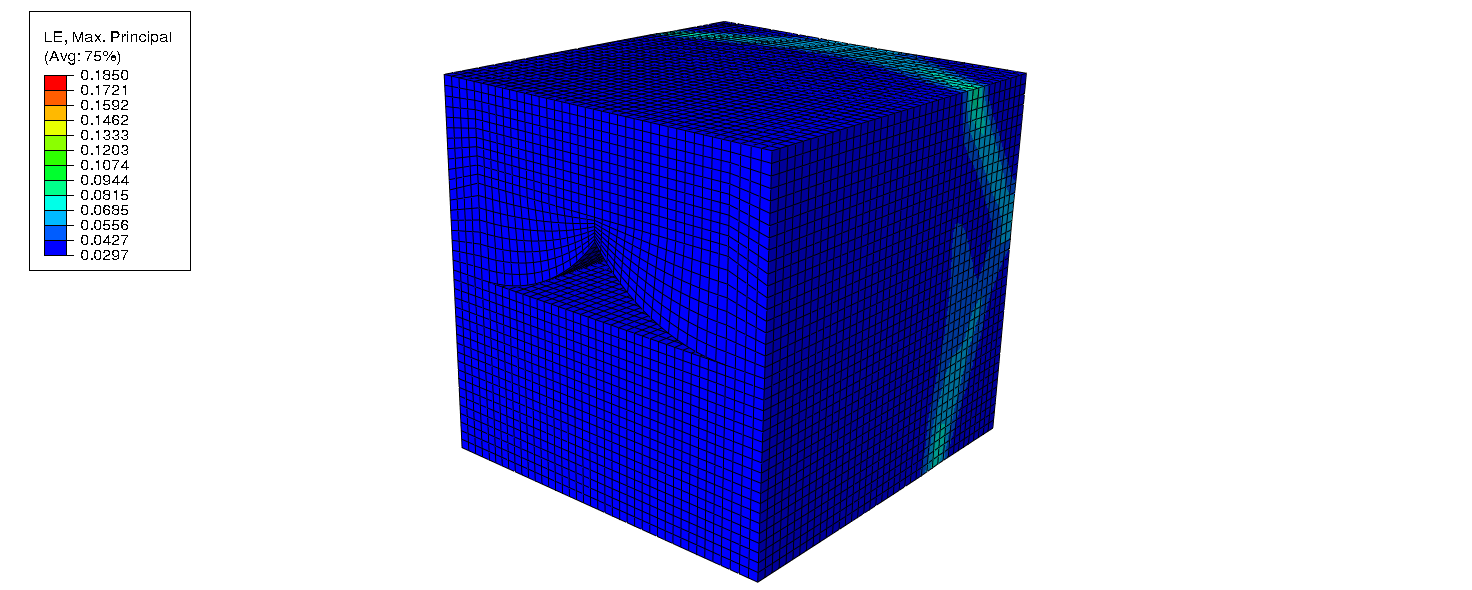
\includegraphics[width=\textwidth]{chapter_7_non-elasticmodelling/figures/1p1.png}
    \caption{0.5 aspect ratio, 1 direction}
  \end{subfigure}
  \\
    \begin{subfigure}[b]{0.80\textwidth}
    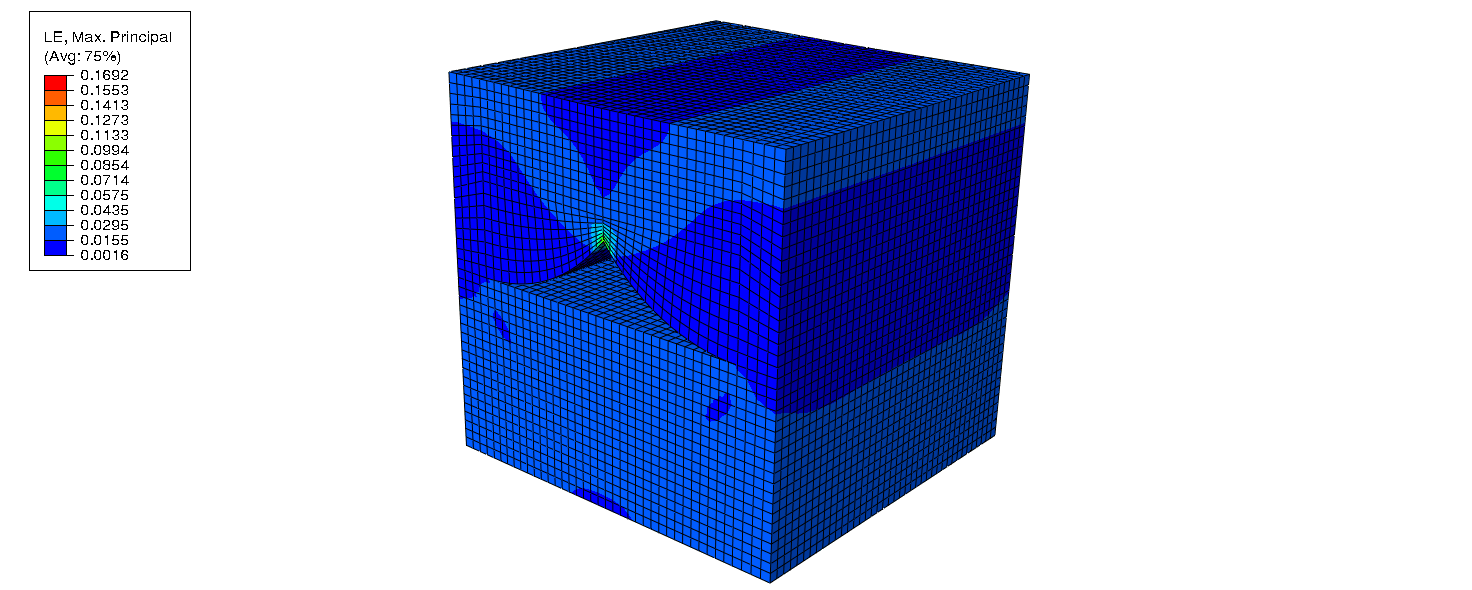
\includegraphics[width=\textwidth]{chapter_7_non-elasticmodelling/figures/1p2.png}
    \caption{0.5 aspect ratio, 2 direction}
  \end{subfigure}
  \\
  \begin{subfigure}[b]{0.80\textwidth}
    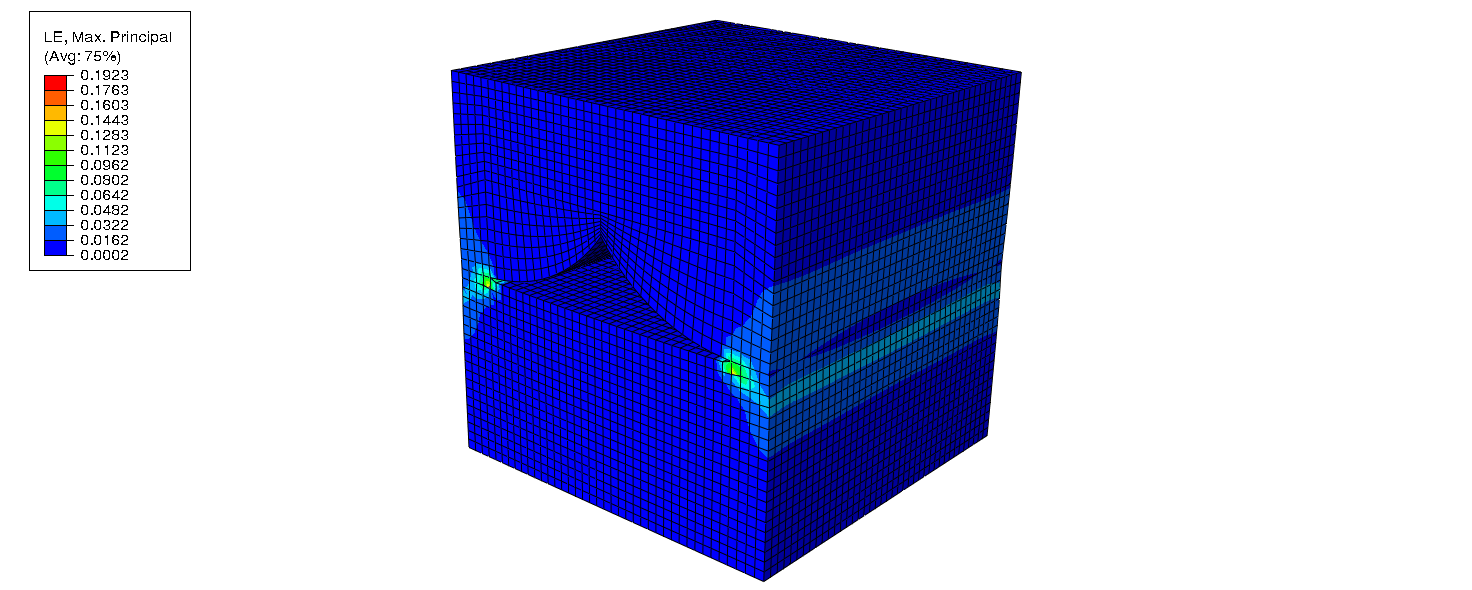
\includegraphics[width=\textwidth]{chapter_7_non-elasticmodelling/figures/1p3.png}
    \caption{0.5 aspect ratio, 3 direction}
  \end{subfigure}
  \caption{Contour plots of different aspect ratios just before failure}
  \label{fig:Contourplot}
\end{figure}

\subsection{Comparison fracture stress}

\begin{figure}[H]
    \centering
    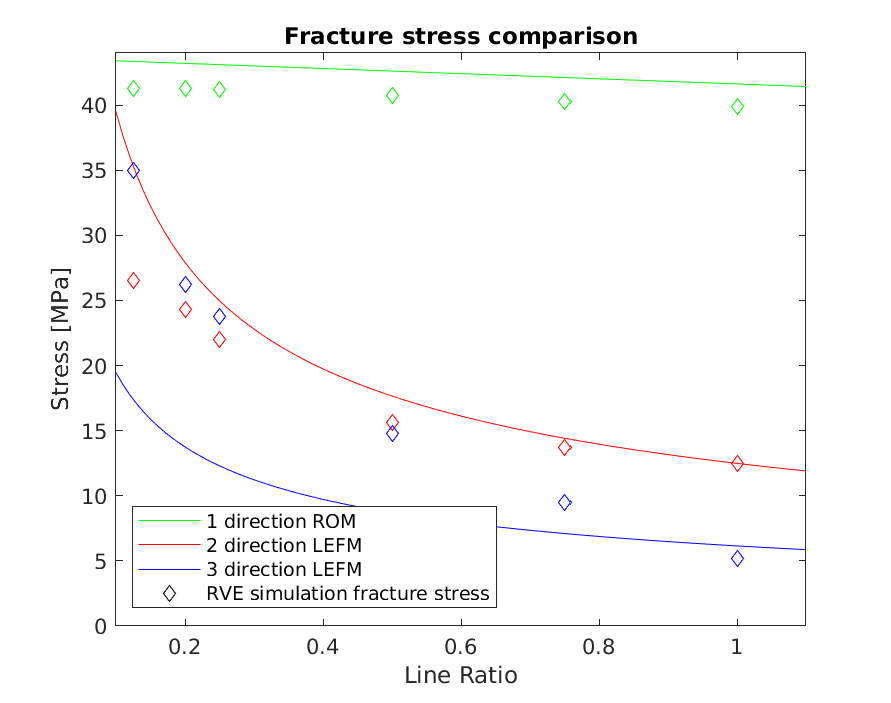
\includegraphics[width=0.80\textwidth]{chapter_7_non-elasticmodelling/figures/yieldstress.png}
    \caption{Comparison between fracture stress of the Stress Intensity approach and the RVE simulations for different aspect ratios}
    \label{fig:ComparisonSS}
\end{figure}

\section{Discussion}

\section{Conclusion}

%wait to write after discussion with Miguel

%Interesting to notice is that RVE part should first plastically (ductile failure) deform before rupture (graph), but this doesn't happen since bad inrter layer bonding. 


